\documentclass[12pt]{article}

\usepackage{sbc-template}
\usepackage{graphicx,url}
\usepackage[utf8]{inputenc}
\usepackage[T1]{fontenc}
\usepackage[brazil]{babel}
\usepackage{booktabs,multirow,amsmath}
\usepackage{tikz}
\usetikzlibrary{positioning,arrows.meta}
\usepackage[hidelinks]{hyperref}

\sloppy

\title{Detecção de Intrusões por Anomalia em Tráfego GOOSE\\
com MLP e Random Forest: Base para um IDS Híbrido\\ com Regras Geradas por LLM}

\author{
Lucas A. Martins\inst{1},
Camilla B. Quincozes\inst{1}, Giovanni Siervo\inst{1},\\
Silvio E. Quincozes\inst{1,2}, Éderson Rosa da Silva\inst{1}
}

% [CONFIRMAR] identificadores de e-mail e se todos são @ufu.br.
\address{Universidade Federal de Uberlândia (UFU) --
Uberlândia, Brasil
\nextinstitute
Universidade Federal do Pampa (UNIPAMPA) --
Alegrete, Brasil
\email{\{lucas.martins, camillaquincozes, gsiervo, sequincozes, ersilva\}@ufu.br}}

\begin{document}

\maketitle

\begin{abstract}
GOOSE messages (IEC 61850) carry protection commands in digital substations
without native authentication. Signature rules generated by LLMs are
interpretable and cheap, but only cover known behaviors. This paper builds the
anomaly module of a hybrid IDS, comparing a Multilayer Perceptron (MLP) and a
Random Forest (RF) on the ERENO \textit{dataset} (199,998 messages, 9 classes). RF
achieved 92.41\% accuracy and 93.49\% macro-F1, while the MLP reached 89.98\%
and 91.09\% with 0.20~ms per-message inference. Both detect over 99.7\% of
masquerade, injection and state-number poisoning attacks; grayhole and random
replay remain the hardest. Combining the models with high-precision LLM rules
is the basis of the proposed hybrid IDS.
\end{abstract}

\begin{resumo}
Mensagens GOOSE (IEC 61850) transportam comandos de proteção em subestações
digitais sem autenticação nativa. Regras de assinatura geradas por LLMs são
interpretáveis e baratas, mas cobrem apenas comportamentos conhecidos. Este
artigo constrói o módulo de anomalia de um IDS híbrido, comparando um
\textit{Multilayer Perceptron} (MLP) e um \textit{Random Forest} (RF) no
\textit{dataset} ERENO (199.998 mensagens, 9 classes). O RF obteve 92,41\% de acurácia
e 93,49\% de F1-macro; o MLP, 89,98\% e 91,09\%, com inferência de 0,20~ms por
mensagem. Ambos detectam mais de 99,7\% dos ataques de falsificação, injeção e
envenenamento de contadores de estado; \textit{grayhole} e \textit{replay}
aleatório permanecem os mais difíceis. A combinação com regras LLM de alta
precisão fundamenta o IDS híbrido proposto.
\end{resumo}

\section{Introdução}

A norma IEC 61850 padroniza a comunicação em subestações digitais, e o
protocolo GOOSE (\textit{Generic Object Oriented Substation Event}) é o
responsável pela troca de eventos críticos entre dispositivos eletrônicos
inteligentes (IEDs), como comandos de abertura de disjuntores, com requisitos
de latência de até 4~ms~\cite{iec61850-8-1}. Para cumprir esse prazo, o GOOSE é
transmitido em \textit{multicast} na camada de enlace e, na prática, sem
autenticação nem cifragem, já que os mecanismos da IEC~62351-6 raramente são
implantados~\cite{iec62351-6,quincozes2021survey}. Isso abre espaço para
ataques de injeção, \textit{replay}, falsificação do publicador e negação de
serviço já demonstrados na
literatura~\cite{hoyos2012exploiting,kush2014poisoned,boeding2023testbed}.

Sistemas de Detecção de Intrusão (IDSs) baseados em especificação dominam o
cenário de subestações por serem leves e
interpretáveis~\cite{hong2014integrated,yang2017multidimensional,quincozes2021survey}.
No SBRC~2026, propusemos um \textit{pipeline} que usa um LLM para extrair
\textit{red flags} de amostras rotuladas e convertê-las automaticamente em
regras de detecção~\cite{martins2026redflags}. Regras, porém, só reconhecem o
que descrevem. Comportamentos sutis, como o descarte seletivo de mensagens
(\textit{grayhole}) ou o reenvio de quadros legítimos, exigem um modelo que
aprenda o perfil do tráfego.

Este trabalho constrói essa segunda metade: um módulo de detecção por anomalia
baseado em redes neurais, que será combinado às regras geradas por LLM em um
IDS híbrido. As contribuições são:
(i) uma ferramenta em \textit{notebook}, reprodutível, que permite escolher a
base de dados e o algoritmo (MLP ou RF), treinar, testar e gerar matrizes de
confusão e gráficos por classe de ataque e por falha de segurança do GOOSE;
(ii) uma comparação experimental entre MLP e RF no \textit{dataset}
ERENO~\cite{quincozes2024ereno}; e
(iii) uma primeira avaliação da fusão entre o modelo de anomalia e as regras
do SBRC~2026, com uma estratégia de seleção de regras que evita falsos
positivos.

\section{Trabalhos Relacionados}

Modelos supervisionados são a abordagem mais comum para GOOSE.
Bhattacharya et al.~\cite{bhattacharya2024ml} e
Senel e Al-Hubaishi~\cite{senel2026simultaneous} reportam
acurácias acima de 99\% com \textit{ensembles}, enquanto
Yasseen e Csatár~\cite{yasseen2026optimal} mostram que a
escolha de atributos temporais domina o desempenho. No ERENO,
Moore~\cite{moore2026anomaly} compara um RF
supervisionado (F1 de 0,95) com \textit{autoencoders} recorrentes, e observa que o RF
não atende ao limite de 4~ms por predição. Abordagens não supervisionadas usam
\textit{autoencoders} explicáveis~\cite{lozano2026explainable} e
\textit{transformers}~\cite{goyel2026transformer}, e o GOOSEIDRS associa
LightGBM a respostas automáticas contra falsificação~\cite{alberto2026gooseidrs}.
LLMs vêm sendo aplicados diretamente à detecção~\cite{zaboli2025genai,danso2025llm}
e à geração de regras~\cite{hadi2026genti,martins2026redflags}. Arquiteturas
híbridas regra + aprendizado aparecem em \cite{girdhar2024sdn,yoon2025sdn},
mas com regras escritas manualmente. Até onde sabemos, este é o primeiro
trabalho a combinar um modelo de anomalia com regras \emph{geradas por LLM}
para GOOSE.

\section{Proposta: IDS Híbrido}

A Figura~\ref{fig:arq} resume a arquitetura. O tráfego GOOSE é espelhado e os
atributos são extraídos por mensagem. Dois módulos operam em paralelo: o
\textbf{módulo de assinatura} aplica as regras geradas pelo LLM no SBRC~2026,
interpretáveis e implementáveis em planos de dados programáveis
(P4)~\cite{bosshart2014p4,fida2026pdpsurvey}; o \textbf{módulo de anomalia},
objeto deste artigo, classifica a mensagem com MLP ou RF. A fusão emite um
alerta quando o modelo ou uma regra \emph{selecionada} dispara (Seção~\ref{sec:hib}).

\begin{figure}[ht]
\centering
\resizebox{\linewidth}{!}{% Diagrama da arquitetura do IDS hibrido (TikZ) -- incluido via % Diagrama da arquitetura do IDS hibrido (TikZ) -- incluido via % Diagrama da arquitetura do IDS hibrido (TikZ) -- incluido via \input{arquitetura}
\begin{tikzpicture}[
  font=\footnotesize, >=Stealth, node distance=4mm and 6mm,
  box/.style={draw=black!60, rounded corners=2pt, align=center, minimum height=9mm, inner sep=3pt, fill=white},
  sig/.style={box, fill=green!8}, ano/.style={box, fill=blue!8}, dec/.style={box, fill=violet!10},
  lbl/.style={font=\scriptsize\itshape, text=black!65}]
  \node[box, minimum width=22mm] (in) {Tr\'afego GOOSE\\(espelhamento / TAP)};
  \node[box, right=of in, minimum width=22mm] (pre) {Extra\c{c}\~ao de\\atributos};
  \node[sig, above right=3mm and 8mm of pre, minimum width=36mm] (sig)
       {\textbf{M\'odulo de assinatura}\\regras geradas por LLM\\(SBRC 2026)};
  \node[ano, below right=3mm and 8mm of pre, minimum width=36mm] (ano)
       {\textbf{M\'odulo de anomalia}\\MLP ou Random Forest\\(este trabalho)};
  \node[dec, anchor=west, minimum width=24mm] (fus) at ([xshift=12mm]sig.east |- pre.east) {\textbf{Fus\~ao}\\OU seletivo};
  \node[box, right=of fus, minimum width=20mm] (out) {Alerta /\\bloqueio};
  \draw[->] (in) -- (pre);
  \draw[->] (pre.east) -- ++(3mm,0) |- (sig.west);
  \draw[->] (pre.east) -- ++(3mm,0) |- (ano.west);
  \draw[->] (sig.east) -- ++(5mm,0) |- (fus.west);
  \draw[->] (ano.east) -- ++(5mm,0) |- (fus.west);
  \draw[->] (fus) -- (out);
  \node[lbl, above=0.5mm of sig] {ataques conhecidos, interpret\'avel, plano de dados (P4)};
  \node[lbl, below=0.5mm of ano] {desvios do comportamento normal aprendido};
\end{tikzpicture}

\begin{tikzpicture}[
  font=\footnotesize, >=Stealth, node distance=4mm and 6mm,
  box/.style={draw=black!60, rounded corners=2pt, align=center, minimum height=9mm, inner sep=3pt, fill=white},
  sig/.style={box, fill=green!8}, ano/.style={box, fill=blue!8}, dec/.style={box, fill=violet!10},
  lbl/.style={font=\scriptsize\itshape, text=black!65}]
  \node[box, minimum width=22mm] (in) {Tr\'afego GOOSE\\(espelhamento / TAP)};
  \node[box, right=of in, minimum width=22mm] (pre) {Extra\c{c}\~ao de\\atributos};
  \node[sig, above right=3mm and 8mm of pre, minimum width=36mm] (sig)
       {\textbf{M\'odulo de assinatura}\\regras geradas por LLM\\(SBRC 2026)};
  \node[ano, below right=3mm and 8mm of pre, minimum width=36mm] (ano)
       {\textbf{M\'odulo de anomalia}\\MLP ou Random Forest\\(este trabalho)};
  \node[dec, anchor=west, minimum width=24mm] (fus) at ([xshift=12mm]sig.east |- pre.east) {\textbf{Fus\~ao}\\OU seletivo};
  \node[box, right=of fus, minimum width=20mm] (out) {Alerta /\\bloqueio};
  \draw[->] (in) -- (pre);
  \draw[->] (pre.east) -- ++(3mm,0) |- (sig.west);
  \draw[->] (pre.east) -- ++(3mm,0) |- (ano.west);
  \draw[->] (sig.east) -- ++(5mm,0) |- (fus.west);
  \draw[->] (ano.east) -- ++(5mm,0) |- (fus.west);
  \draw[->] (fus) -- (out);
  \node[lbl, above=0.5mm of sig] {ataques conhecidos, interpret\'avel, plano de dados (P4)};
  \node[lbl, below=0.5mm of ano] {desvios do comportamento normal aprendido};
\end{tikzpicture}

\begin{tikzpicture}[
  font=\footnotesize, >=Stealth, node distance=4mm and 6mm,
  box/.style={draw=black!60, rounded corners=2pt, align=center, minimum height=9mm, inner sep=3pt, fill=white},
  sig/.style={box, fill=green!8}, ano/.style={box, fill=blue!8}, dec/.style={box, fill=violet!10},
  lbl/.style={font=\scriptsize\itshape, text=black!65}]
  \node[box, minimum width=22mm] (in) {Tr\'afego GOOSE\\(espelhamento / TAP)};
  \node[box, right=of in, minimum width=22mm] (pre) {Extra\c{c}\~ao de\\atributos};
  \node[sig, above right=3mm and 8mm of pre, minimum width=36mm] (sig)
       {\textbf{M\'odulo de assinatura}\\regras geradas por LLM\\(SBRC 2026)};
  \node[ano, below right=3mm and 8mm of pre, minimum width=36mm] (ano)
       {\textbf{M\'odulo de anomalia}\\MLP ou Random Forest\\(este trabalho)};
  \node[dec, anchor=west, minimum width=24mm] (fus) at ([xshift=12mm]sig.east |- pre.east) {\textbf{Fus\~ao}\\OU seletivo};
  \node[box, right=of fus, minimum width=20mm] (out) {Alerta /\\bloqueio};
  \draw[->] (in) -- (pre);
  \draw[->] (pre.east) -- ++(3mm,0) |- (sig.west);
  \draw[->] (pre.east) -- ++(3mm,0) |- (ano.west);
  \draw[->] (sig.east) -- ++(5mm,0) |- (fus.west);
  \draw[->] (ano.east) -- ++(5mm,0) |- (fus.west);
  \draw[->] (fus) -- (out);
  \node[lbl, above=0.5mm of sig] {ataques conhecidos, interpret\'avel, plano de dados (P4)};
  \node[lbl, below=0.5mm of ano] {desvios do comportamento normal aprendido};
\end{tikzpicture}
}
\caption{Arquitetura do IDS híbrido proposto.}
\label{fig:arq}
\end{figure}

\section{Metodologia}

\textbf{Dataset.} Usamos o ERENO-2.0-100K~\cite{quincozes2024ereno}: 199.998
mensagens GOOSE após a remoção de 54 linhas de cabeçalho ARFF, sendo 39.999
normais e cerca de 20 mil de cada um de oito ataques (\textit{grayhole},
\textit{high\_StNum}, \textit{injection}, \textit{inverse\_replay},
\textit{masquerade\_fake\_fault}, \textit{masquerade\_fake\_normal},
\textit{poisoned\_high\_rate} e \textit{random\_replay}).
Onze colunas categóricas são constantes e foram descartadas, assim como os
carimbos de tempo absolutos (\texttt{Time}, \texttt{t},
\texttt{GooseTimestamp}), para evitar que o modelo memorize a ordem da
simulação. Restaram 37 atributos: 19 do cabeçalho GOOSE e derivados
(\texttt{StNum}, \texttt{SqNum}, \texttt{stDiff}, \texttt{timestampDiff},
\texttt{timeFromLastChange} etc.) e 18 medidas elétricas do barramento.

\textbf{Modelos.} O MLP~\cite{rumelhart1986learning,haykin2009neural} tem duas
camadas ocultas (128 e 64 neurônios, ReLU), otimizador
Adam~\cite{kingma2015adam}, regularização L2 ($10^{-4}$), lotes de 256 e
\textit{early stopping} em 10\% do treino; convergiu em 80 épocas. O
RF~\cite{breiman2001random} usa 100 árvores sem poda (Gini). As entradas do MLP
são padronizadas com média e desvio do treino. Ambos foram implementados em
scikit-learn~\cite{pedregosa2011scikit}, com divisão estratificada 70/30
(139.998/60.000 mensagens) e semente fixa (42).

\textbf{Ferramenta.} O \textit{notebook}
\texttt{IDS\_GOOSE\_Anomalia\_MLP\_RF.ipynb} segue a estrutura do artefato do
SBRC~2026: o usuário define o \textit{dataset} (\texttt{DATASET}) e o algoritmo
(\texttt{ALGORITMO} = MLP, RF ou AMBOS), e o \textit{notebook} executa a
limpeza, o treino, o teste, as matrizes de confusão, os gráficos por classe e
por falha GOOSE, o comparativo e a fusão híbrida, exportando figuras e CSVs.

\textbf{Métricas.} Reportamos acurácia, precisão, \textit{recall} e F1
(macro) na tarefa de 9 classes e, na visão binária normal $\times$ ataque,
taxa de detecção (TPR) e de falsos positivos (FPR).

\section{Resultados}

A Tabela~\ref{tab:res} resume o desempenho. O RF supera o MLP em todas as
métricas de qualidade (+2,4 pontos de F1-macro), mas o MLP é 26 vezes mais
rápido na inferência unitária: 0,20~ms contra 5,3~ms por mensagem, medidos com
uma \textit{thread}. Em lote, o custo cai para 2,7~$\mu$s (MLP) e 8,7~$\mu$s
(RF) por mensagem, o que mostra que a latência unitária do RF reflete sobretudo
o custo de percorrer 100 árvores em Python, e não um limite do modelo.

\begin{table}[ht]
\centering
\caption{Desempenho no conjunto de teste (60.000 mensagens).}
\label{tab:res}
\small
\begin{tabular}{lcccccccc}
\toprule
& \multicolumn{4}{c}{9 classes (macro)} & \multicolumn{2}{c}{Normal $\times$ ataque} & \multicolumn{2}{c}{Custo}\\
\cmidrule(lr){2-5}\cmidrule(lr){6-7}\cmidrule(lr){8-9}
Modelo & Acur. & Prec. & Rec. & F1 & TPR & FPR & Treino & Inferência\\
\midrule
MLP & 89,98 & 91,84 & 90,66 & 91,09 & 93,53 & 16,12 & 64~s & 0,20~ms\\
RF  & \textbf{92,41} & \textbf{94,11} & \textbf{93,03} & \textbf{93,49} & \textbf{93,95} & \textbf{13,11} & 24~s & 5,3~ms\\
\bottomrule
\end{tabular}
\end{table}

A Figura~\ref{fig:cm} mostra que os erros se concentram em dois pares. O
primeiro é \textit{grayhole} $\leftrightarrow$ normal: no RF, 36,6\% das
mensagens de \textit{grayhole} foram classificadas como normais e 12,2\% das
normais como \textit{grayhole}. Isso é esperado, pois o \textit{grayhole}
descarta mensagens seletivamente, e as que chegam são legítimas; a evidência
do ataque está na \emph{ausência} de mensagens, que uma análise por mensagem
isolada não observa. O segundo par é \textit{random\_replay} $\to$ normal
(11,7\% no RF e 22,3\% no MLP), já que o quadro reenviado é uma cópia de um
quadro válido.

\begin{figure}[ht]
\centering
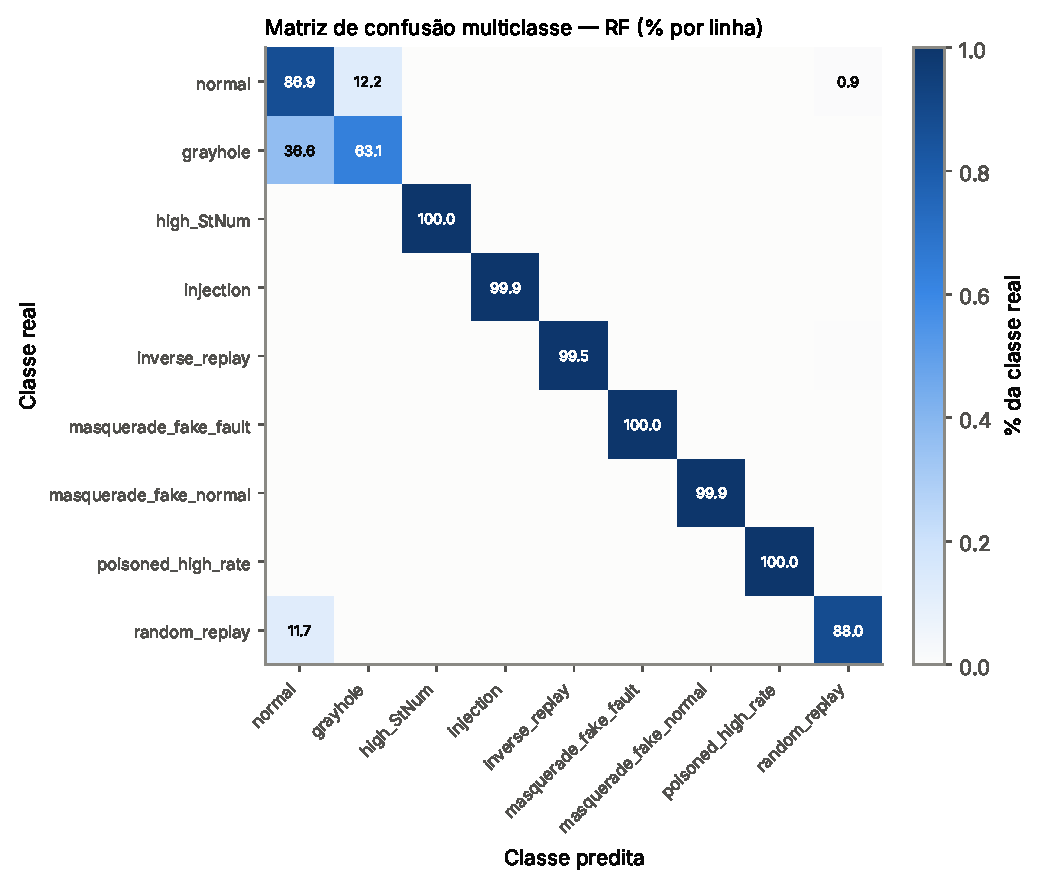
\includegraphics[width=0.6\linewidth]{figuras/fig03_cm_multiclasse_RF.pdf}
\caption{Matriz de confusão do Random Forest (\% por classe real).}
\label{fig:cm}
\end{figure}

A Figura~\ref{fig:falhas} agrega as detecções pela falha de segurança do GOOSE
explorada por cada ataque. As falhas de autenticação de origem (F1),
integridade (F2) e validação de \texttt{stNum}/\texttt{sqNum} (F4) são
cobertas em mais de 99,7\% pelos dois modelos. A ausência de proteção
anti-\textit{replay} (F3) é coberta em 94,1\% pelo RF e 88,7\% pelo MLP; a
ausência de garantia de entrega (F5, \textit{grayhole}) é a lacuna mais
difícil, com 63,4\% (RF) e 71,4\% (MLP), o único caso em que o MLP vence. Os
atributos mais relevantes para o RF são \texttt{timeFromLastChange} (15,7\%),
\texttt{StNum} (15,4\%), \texttt{timestampDiff} (9,7\%) e \texttt{SqNum}
(9,1\%), os mesmos campos que fundamentam as \textit{red flags} do
SBRC~2026~\cite{martins2026redflags}. As medidas elétricas, porém, também
contam: sem elas (19 atributos), o F1-macro do RF cai de 93,49\% para 91,36\%
e o FPR sobe para 16,37\%, sobretudo por causa do \textit{random\_replay}.

\begin{figure}[ht]
\centering
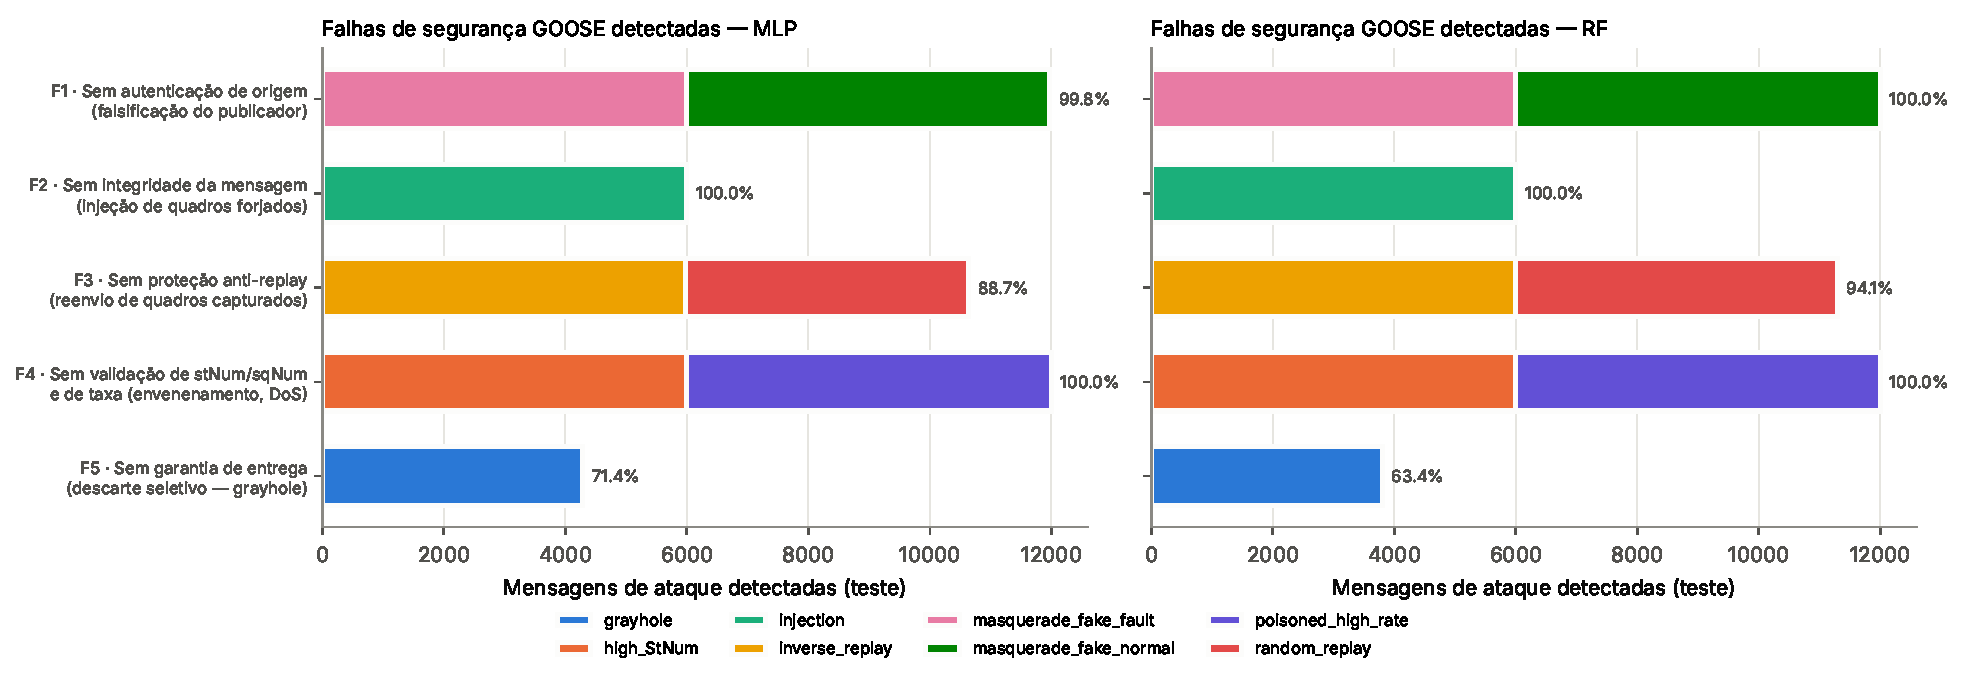
\includegraphics[width=\linewidth]{figuras/fig06_falhas_goose.pdf}
\caption{Mensagens de ataque detectadas por falha de segurança do GOOSE
(percentual = cobertura da falha no teste).}
\label{fig:falhas}
\end{figure}

\subsection{Fusão com as regras geradas por LLM}\label{sec:hib}

As 22 regras do SBRC~2026 foram aplicadas ao mesmo conjunto de teste. Isoladas,
elas alcançam TPR de 32,58\% com FPR de 5,01\% (Tabela~\ref{tab:hib}). Uma fusão
OU ingênua com o RF quase não aumenta a detecção (+0,12 ponto) e eleva o FPR
de 13,11\% para 17,90\%. Por isso, propomos a \textbf{fusão seletiva}: apenas as
regras com FPR $\le$ 0,5\% em tráfego normal, \emph{medido no treino}, entram
na fusão. Dezesseis regras foram selecionadas, com FPR de 1,26\% no teste, e o
híbrido seletivo mantém o ganho de detecção limitando o FPR adicional a 1,15
ponto. As regras custam cerca de 2,7~$\mu$s por mensagem.

\begin{table}[ht]
\centering
\caption{Visão binária normal $\times$ ataque: modelos, regras LLM e fusões (\%).}
\label{tab:hib}
\small
\begin{tabular}{lcccc}
\toprule
Configuração & TPR & FPR & Precisão & F1\\
\midrule
Regras LLM (todas, 22)        & 32,58 & 5,01  & 96,30 & 48,69\\
Regras LLM (selecionadas, 16) & 29,57 & 1,26  & 98,95 & 45,53\\
RF                            & 93,95 & 13,11 & 96,63 & 95,27\\
Híbrido OU (RF + todas)       & 94,07 & 17,90 & 95,46 & 94,76\\
Híbrido seletivo (RF + 16)    & 94,04 & 14,26 & 96,35 & 95,18\\
\bottomrule
\end{tabular}
\end{table}

O resultado mostra que, neste \textit{dataset}, o modelo supervisionado já captura quase
todos os ataques que as regras cobrem. O valor das regras no IDS híbrido está
em outra dimensão: interpretabilidade, custo de microssegundos e a possibilidade
de execução no plano de dados~\cite{xavier2021programmable}, o que viabiliza um
arranjo em cascata, no qual as regras filtram ataques conhecidos na taxa de
linha e o modelo trata o restante.

\section{Conclusão}

Este artigo apresentou o módulo de anomalia de um IDS híbrido para GOOSE e uma
ferramenta reprodutível para treiná-lo e avaliá-lo. O Random Forest foi o
modelo mais preciso (F1-macro de 93,49\%), e o MLP, o mais adequado ao
requisito de 4~ms (0,20~ms por mensagem). As duas falhas que permanecem abertas,
falta de garantia de entrega e de proteção anti-\textit{replay}, dependem do
contexto entre mensagens. Como trabalhos futuros, propomos atributos de janela
temporal e modelos sequenciais para \textit{grayhole} e \textit{replay}, o
arranjo em cascata regras $\to$ modelo no Intel Tofino e a avaliação de
generalização em ataques não vistos no treino.

\bibliographystyle{sbc}
\bibliography{referencias}

\end{document}
